\documentclass[12pt]{article}
%\usepackage{natbib}
\usepackage[french]{babel}
\usepackage{url}
\usepackage[utf8x]{inputenc}
\usepackage{graphicx}
\graphicspath{{images/}}
\usepackage{parskip}
\usepackage{fancyhdr}
\usepackage{vmargin}
\usepackage{xcolor}
\usepackage{bbm}
\usepackage{amsmath,amsthm,amssymb,latexsym,amsfonts}
\usepackage{dsfont}
\usepackage{stmaryrd}
\usepackage{systeme}
\usepackage{enumitem}
\usepackage{pifont}
%\usepackage[cache=false]{minted}
%\definecolor{LightGray}{gray}{0.95}
\usepackage{autobreak}
\usepackage{hyperref}
\usepackage{tikz}

\title{Théorème fondamental des polynômes symétriques}
\author{PIARD A. - JACQUET R. - CARVAILLO T.}
\date{\today}

\makeatletter
\let\thetitle\@title
\let\theauthor\@author
\let\thedate\@date
\makeatother

\pagestyle{fancy}
\fancyhf{}
\rhead{\fontsize{7}{7} \selectfont \theauthor}
\lhead{\fontsize{10}{10} \selectfont \thetitle}
\cfoot{\thepage}
\def\dotfill#1{\cleaders\hbox to #1{.}\hfill}
\newcommand\dotline[2][.5em]{\leavevmode\hbox to #2{\dotfill{#1}\hfil}}

%définition commande présentation fonction
\newcommand{\fonction}[5]{
\begin{displaymath}
\begin{array}{l|rcl}
\displaystyle
#1 : & #2 & \longrightarrow & #3 \\
    & #4 & \longmapsto & #5
\end{array}
\end{displaymath}
}
%fin définition
\theoremstyle{remark}\newtheorem{note}{Note}
\theoremstyle{remark}\newtheorem{nota}{Notation}

\newcommand{\M}{\mathbbm{M}}
\newcommand{\N}{\mathbbm{N}}
\newcommand{\Z}{\mathbbm{Z}}
\newcommand{\Q}{\mathbbm{Q}}
\newcommand{\R}{\mathbbm{R}}
\newcommand{\C}{\mathbbm{C}}
\newcommand{\G}{\mathbbm{G}}
\newcommand{\K}{\mathbbm{K}}
\newcommand{\F}{\mathbbm{F}}
\newcommand{\Fq}{\mathbbm{F}_q}
\newcommand{\Fqn}{\mathbbm{F}_{q^n}}
\newcommand{\Fp}{\mathbbm{F}_p}
\newcommand{\ord}{\preccurlyeq}

%fin définition


% de jolies accolades
\newcommand{\accolade}[2]{
\begin{displaymath}
%#1 = \left\{
    \begin{array}{ll}
       #1 %& \mbox{si }
       #2 %& \mbox{sinon.}
    \end{array}
\right.
\end{displaymath}
}
% de jolies accolades


\newtheorem{theorem}{Théorème}
\newtheorem{corollaire}{Corollaire}
\newtheorem{lemma}{Lemme}
\newtheorem{prop}{Proposition}
\theoremstyle{definition}
\newtheorem{definition}{Définition}
\newtheorem{example}{Exemple}
\newtheorem*{examples}{Exemples}
\newtheorem{exo}{Exercice}	
\newtheorem{coro}{Corollaire}	
\newtheorem{rem}{Remarque}
\newtheorem{crit}{Critère}
\newtheorem{bg}{A l'attention des bg, question}

\newtheorem{thm}{Theorem}
\newcommand{\statetheoremhoriz}[2][\textwidth]{
 \par\noindent\tikzstyle{mybox} = [draw=black,left color=gray!30,
  right color=gray!7,thick,rectangle,inner sep=6pt]
 \begin{tikzpicture}
  \node [mybox] (box){%
   \begin{minipage}{#1}{#2}\end{minipage}
  };
 \end{tikzpicture}
}
\newcommand{\statetheoremvert}[2][\textwidth]{
 \par\noindent\tikzstyle{mybox} = [draw=blue,top color=cyan!50,
  bottom color=cyan!5,thick,rectangle,inner sep=6pt]
 \begin{tikzpicture}
  \node [mybox] (box){%
   \begin{minipage}{#1}{#2}\end{minipage}
  };
 \end{tikzpicture}
}
\newcommand{\statetheoremsolid}[2][\textwidth]{
 \par\noindent\tikzstyle{mybox} = [draw=blue,fill=cyan!50,
  thick,rectangle,inner sep=6pt]
 \begin{tikzpicture}
  \node [mybox] (box){%
   \begin{minipage}{#1}{#2}\end{minipage}
  };
 \end{tikzpicture}
}

\begin{document}
%%%%%%%%%%%%%%%%%%%%%%%%%%%%%%%%%%%%%%%%%%%%%%%%%%%%%%%%%%%%%%%%%%%%%%%%%%%%%%%%%%%%%%%%%

\begin{titlepage}
	\centering
    \vspace*{0.5 cm}
    \textsc{\LARGE Projet de Systèmes Polynomiaux.\\
    \vspace{12pt}
2020-2021}\\[1.0 cm]
    \dotline[15pt]{15cm}\\
	
\includegraphics[scale = 2.2]{logo.png}
	\dotline[15pt]{15cm}\\
	\vspace{1.5cm}
	\textsc{\Large Faculté des Sciences et Techniques}\\
	\textsc{\large Master 1 - Maths. CRYPTIS}\\[1.0 cm]
	\rule{\linewidth}{0.2 mm} \\[0.4 cm]
	{ \huge \bfseries \color{blue} \thetitle}\\
	\rule{\linewidth}{0.2 mm} \\[1.5 cm]
	
	\begin{minipage}{0.4\textwidth}
		\begin{flushleft} \large
			\emph{A l'attention de :}\\
			M. LICKTEIG\\
			\phantom{a}\\
			\phantom{a}\\
		\end{flushleft}
	\end{minipage}
	\begin{minipage}{0.5\textwidth}
    	\begin{flushright} \large
		\emph{Rédigé par :}\\
		PIARD A.\\
		JACQUET R.\\
		CARVAILLO T.\\
		\end{flushright}
	\end{minipage}\\[2 cm]
\end{titlepage}

%%%%%%%%%%%%%%%%%%%%%%%%%%%%%%%%%%%%%%%%%%%%%%%%%%%%%%%%%%%%%%%%%%%%%%%%%%%%%%%%%%%%%%%%%

\tableofcontents
\pagebreak

\section{Polynômes multivariés}


\statetheoremhoriz{
\begin{definition}[Ordre]
Soit $E$ un ensemble quelconque, on appelle \textit{ordre partiel} sur $E$ toute relation vérifiant les propriétés suivantes pour $(x,y) \in E^2$:
	 \begin{enumerate}
	 	\item $x\ord x$ (réflexivité)
	 	\item $x\ord y$ et $y\ord x \Rightarrow x=y$ (antisymétrie)
	 	\item $x\ord y$ et $y\ord z \Rightarrow x\ord z$ (transitivité)
	 \end{enumerate}
En d'autres terme, $\ord$ est une relation d'équivalence sur $E$.
\end{definition}}
\statetheoremhoriz{
\begin{definition}[Ordre total, ordonné]
Sous les mêmes notations, on dit que $\ord$ est un \textit{ordre total} si deux éléments quelconques sont toujours comparable, i.e. si
	\begin{center}$\forall (x,y)\in E^2, x\ord y\text{ ou } y\ord x$\end{center}
De plus, $\ord$ est dit \textit{bien ordonné} si
	\begin{center}$  \forall\text{ } F \subseteq E, \exists \text{ } f_{min}\in F \text{ tel que } \forall f\in F, \text{ } f_{min}\ord f $\end{center}
\end{definition}}
\statetheoremhoriz{
\begin{definition}[Monoïde]
On appelle monoïde tout ensemble muni d'une loi de composition interne et d'un élément neutre.
\end{definition}}
\statetheoremhoriz{
\begin{definition}
Soient $n\in\N$ et $\{X_1, ..., X_n\}$ un ensemble fini d'indéterminées. On définit le monoïde $\M_n$ comme suit:
	\begin{center} $\M_n := \{ X^{\alpha} := X_1^{\alpha_1}\ldots X_n^{\alpha_n}\}$ \end{center}
\end{definition}}
\statetheoremhoriz{
\begin{prop} Soit,
\fonction{\phi}{\M_n}{\N^n}{ X^{\alpha} := X_1^{\alpha_1}\ldots X_n^{\alpha_n}}{\alpha:=(\alpha_1,\ldots, \alpha_n)}
alors $\phi$ un isomorphisme de monoïde.
\end{prop}}
\statetheoremhoriz{
\begin{definition}[Ordre monomial]
On dit que $\ord$ est un ordre monomial sur $\M_n$ si 
	\begin{enumerate}
		\item $\ord$ est un ordre total
		\item $\ord$ est compatible avec la multiplication, i.e. si pour tout
		\begin{center} $X=X_1\ldots X_n  \text{ , } \alpha=(\alpha_1,\ldots, \alpha_n) \text{ , } \beta=(\beta_1,\ldots, \beta_n) \text{ et } \gamma=(\gamma_1,\ldots, \gamma_n)$\end{center}
on a 
		\begin{center}$X^{\alpha} \ord X^{\beta }\Rightarrow X^{\alpha}.X^{\gamma} \ord X^{\beta}.X^{\gamma}$\end{center}
		\item $\M_n$ est bien ordonné par $\ord$
	\end{enumerate}
\end{definition}}
\statetheoremhoriz{
\begin{definition}[Ordre lexicographique]
Pour deux vecteurs exposant $\alpha=(\alpha_1,\ldots, \alpha_n) \text{ et } \beta=(\beta_1,\ldots, \beta_n) \in\N^n$, on peut spécifier ordre, appellé \textit{ordre lexicographique} définit comme suit:
	\begin{center} $\alpha\ord_{lex} \beta $\end{center}
	\begin{center} si \end{center}
	\begin{center} $\exists \text{ } m\in\llbracket 1,n \rrbracket \text{ tel que } \forall \text{ } i<m \text{ , } \alpha_i-\beta_i=0  \text{ et } \alpha_m < \beta_m$ \end{center}
\end{definition}}

Nous allons dès à présent travailler dans $\K[X_1, \ldots, X_n]$, et $\ord$ désignera toujours un ordre monomial sur $\M_n\subseteq \K[X_1, \ldots, X_n]$.
\statetheoremhoriz{
\begin{definition}[\textsc{Leading Term}]
On appelle \textit{terme} tout éléments de $\M_n$ multiplié par un élément non nul $c$ du corps de base. \newline
On appelle \textsc{Leading Term}(LT) de $P\in \K[X_1, \ldots, X_n]$, son monôme de plus haut degré par rapport à l'ordre $\ord$. \newline
La constante $c$ sera appelée \textit{Leading Coefficient}(LC), et $X_1^{\alpha_1}\ldots X_n^{\alpha_n}$ le \textit{Leading Monomial}, de sorte que :
\begin{center} $P = \underbrace{\underbrace{c}_\textrm{LC(P)}.\underbrace{X_1^{\alpha_1}\ldots X_n^{\alpha_n}}_\textrm{LM(P)}}_\textrm{LT(P)}$  + Q \end{center}
où $Q\in \K[X_1, \ldots, X_n]$ est constitué des termes de la forme $X^\beta \text{ , } \beta \ord_{lex} \alpha \text{ et } X \in\K[X_1, \ldots, X_n]$.
\end{definition}}
\statetheoremhoriz{
\begin{definition}[Multi degré]
Le vecteur d'exposant $\alpha := (\alpha_1,\ldots, \alpha_n)$ est appellé le multi degré de $P$ et est noté $mdeg(P)$.
\end{definition}}
\statetheoremhoriz{
\begin{prop}
Soient $P,Q \in\K[X_1, \ldots, X_n]$, on a $mdeg(P.Q) = mdeg(P) + mdeg(Q)$.
\end{prop}}

\statetheoremhoriz{
\begin{definition}
On appelle idéal de tête (\textsc{Leading Ideal}) d'un idéal $\mathcal{I} \subset K[X]$ non nul, l'idéal engendré par les LT$(f)$ où $f \in I - \{0\}$,
\begin{align*}
\text{LID}(f) &= \langle \Big\lbrace \textsc{LT}(f) : f \in I - \{ 0 \} \Big\rbrace \rangle\\
&= \langle \Big\lbrace \textsc{LM}(f) : f \in I - \{ 0 \} \Big\rbrace \rangle
\end{align*}
\end{definition}}

\statetheoremhoriz{
\begin{definition}
Soit $I\subseteq \mathbbm{K}[X_1,...,X_n]$ un idéal.\newline
Soit $\preccurlyeq$ un ordre monomial sur $\mathbbm{K}[X_1,...,X_n]$.\newline
$I$ étant de type fini, on peut poser $I=<g_1,\ldots, g_t>$ où les $g_t$ sont tous non nuls.\newline
Soit $G:=(g_1,..., g_t)$.\newline
On dit que $G$ forme une base de \textit{Gröbner} de l'idéal $I$ si
\begin{center}
$\langle \textsc{lt}(g_1),\ldots, \textsc{lt}
(g_t) \rangle = \textsc{lid}(I)$
\end{center}
\end{definition}}


\statetheoremhoriz{
\begin{prop} \vphantom\\
\begin{enumerate}[label=(\roman*)]
\item Pour un ordre monomial $\preccurlyeq$ donné et $I\subseteq \mathbbm{K}[X_1,...,X_n]$ un idéal, il existe toujours une base de \textit{Gröbner}.
\item Toute base de \textit{Gröbner} de $I$ est une base de $I$.
\end{enumerate}
\end{prop}}
\section{Les polynômes symétriques}

\subsection{Introduction aux polynômes symétriques}
Les polynômes symétriques prennent forme à partir de l'étude des racines de n'importe quel polynôme. Considérons le polynôme $P=X^3 + bX^2 + cX + d$. C'est un polynôme cubique donc il a $3$ racines, non nécessairement distinctes. On notera ces racines $\alpha_1 , \alpha_2$ et $\alpha_3$.
Le polynôme $P$ peut alors se factoriser ainsi :
$$X^3 + bX^2 + cX + d = (X - \alpha_1)(X - \alpha_2)(X - \alpha_3),$$
ce qui nous donne :

\begin{align*}
    \left. \begin{array}{ll}
    b & = -(\alpha_3 + \alpha_2 + \alpha_1) \\
        c & = \alpha_2 \alpha_3 + \alpha_1 \alpha_3 + \alpha_1 \alpha_2 \\
       d & = - \alpha_1 \alpha_2 \alpha_3
    \end{array}\right\} (\star)
\end{align*}
On observe donc que les coefficients de $P$ sont polynomiaux en ses racines. Par ailleurs, comme modifier l'ordre des termes de $P$ ne le change pas, il s'ensuit que les polynômes définissant $b,c$ et $d$ par rapport à $\alpha_1$, $\alpha_2$ et $\alpha_3$ restent les mêmes si on permute $\alpha_1$, $\alpha_2$ et $\alpha_3$.\\
Les polynômes respectant ce fait sont dits \textit{polynômes symétriques}. Cela nous amène à la définition générale suivante.\\

%Peut-être réintroduire Sn l'ensemble des permutations à n éléments pour reprendre la definition de la première page de la ref 2
\statetheoremhoriz{
\begin{definition}
Un polynôme $P \in K\left[ X_1, X_2, \ldots , X_n \right] $ est dit symétrique si $$P(X_{i_1}, X_{i_2}, \ldots , X_{i_n}) = P(X_1,X_2,\ldots ,X_n),$$ pour toute permutation $X_{i_1}, X_{i_2}, \ldots , X_{i_n}$ de $X_1,X_2, \ldots ,X_n$.
\end{definition}}
\vspace{12pt}
\begin{examples}
\begin{enumerate}
	\item Soit $P = X^{n} + Y^{n} + Z^{n}\in K\left[ X,Y,Z\right]$, avec $n \in \mathbbm{N}$. Alors $P$ est un polynôme symétrique. Comme le prouve la fonction \textsl{symmfunc} de Maple :\\ 
	
	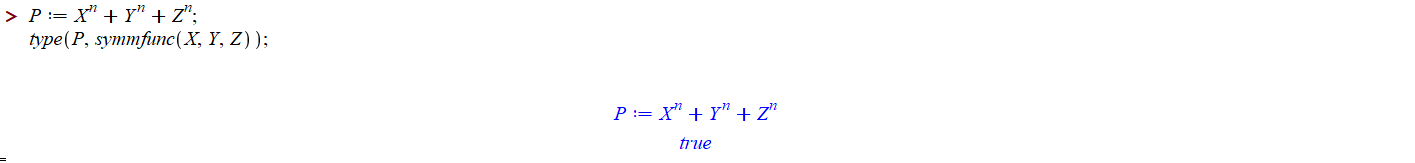
\includegraphics[scale=0.8]{1.png}
Où la fonction renvoie un booléen : \textsl{true} si le polynôme est symétrique, \textsl{false} si non.
	\item Soit $P = XYZ \in K\left[ X,Y,Z\right]$. Ce polynôme est symétrique car $P = XYZ = YZX = ZYX = \ldots$.
\end{enumerate}

\end{examples}

\subsection{Polynômes symétriques élémentaires}
\statetheoremhoriz{
\begin{definition}
Soient $x_1, x_2, ..., x_n$ des variables dans un corps $K$. On définit les fonctions symétriques élémentaires $\sigma_1, ... , \sigma_n \in K[x_1, ..., x_n]$ comme suit,
\begin{align*}
\sigma_1 &= x_1 + ... + x_n \\
& \vdots \\
\sigma_r &=  \displaystyle \sum_{i_1 < i_2 < ... < i_r} x_{i_1} x_{i_2} \cdots x_{i_r}, \\
& \vdots \\
\sigma_n &= x_1 x_2 \cdots x_n
\end{align*}
\end{definition}}

Par conséquent, $\sigma_r$ est la somme de tous les monômes qui sont produits de $r$ variable distinctes. Pour vérifier que les $\sigma_i$, $ i \in \{1, \cdots , n \}$ sont bien symétriques nous allons généraliser le résultat noté $(\star)$ plus haut. On introduit le polynôme,
\begin{center}
$f(X)=(X - x_1)(X-x_2) \cdots (X-x_n) \hspace{0,5cm}, \hspace{0,5cm} (\star \star)$
\end{center}
Ses racines sont donc $x_1, \cdots x_n$. En explicitant le développement de $f(X)$ dont nous vous épargnons les calculs nous obtenons la forme simplifiée suivante
\begin{center}
$f(X) = X^n - \sigma_1 X^{n-1} + \sigma_2 X^{n-2} + \cdots + (-1)^{n-1} \sigma_{n-1} X + (-1)^{n} \sigma_n$
\end{center}
Supposons maintenant que nous réorganisons les $x_i, i \in \{ 1 , \cdots , n \}$. Cela change l'ordre des facteurs de $(\star \star)$ mais la fonction en elle-même reste identique. Donc les coefficients de $(-1)^r \sigma_r$ de la fonction $f$ sont des fonctions symétriques.
\subsection{Le théorème fondamental des polynômes symétriques}
En considérant tous les rappels faits à précédemment, nous pouvons introduire le fameux théorème fondamental des polynômes symétriques.
\statetheoremhoriz{
\begin{theorem}
Tout polynôme symétrique de $K\left[ X_1, X_2, ... , X_n \right]$ peut s'écrire de façon unique comme une expression polynomiale en les polynômes symétriques élémentaires $\sigma_1, \sigma_2,..., \sigma_n$.
\end{theorem}}




\begin{proof}
Pour cette démonstration nous allons utiliser l'ordre lexicographique suivant, $x_1 > x_2 > \ldots > x_n$. Soit $f \in K[x_1, \ldots , x_n]$ un polynôme symétrique non nul, et on définit l'application $LT$ par $LT(f) = ax^{\alpha}$, où $\alpha=(\alpha_1 , \alpha_2, \ldots , \alpha_n )$ et $a \in K$. On peut supposer sans perte de généralité que les $\alpha_i$, $i\in \lbrace 1, \ldots , n \rbrace $ sont ordonnés comme tel : $\alpha_1 \geq \alpha_2 \geq \ldots \geq \alpha_n$.
En effet, supposons que l'on ait $\alpha_i < \alpha_{i+1}$ pour un certain $i\in \lbrace 1, \ldots , n \rbrace $. Il suffit alors de considérer le vecteur d'exposants $\beta$, obtenu à partir de $\alpha$ en permutant $\alpha_i$ et $\alpha_{i+1}$. On écrit $\beta = (\alpha_1 ,\ldots , \alpha_{i+1}, \alpha_i , \ldots , \alpha_n)$. Puisque $ax^{\alpha}$ est un terme de $f$, on en déduit que $ax^{\beta}$ est un terme de $f(x_1 , \ldots , x_{i+1}, x_{i}, \ldots , x_n)$. Or, $f$ est symétrique donc $f(x_1 , \ldots , x_{i+1}, x_{i}, \ldots , x_n)=f$, et par conséquent, $ax^{\beta}$ est un terme de $f$. Ceci est impossible puisque $\beta > \alpha$ selon l'ordre lexicographique.\\

Posons maintenant,
\begin{center}
$h=\sigma_1^{\alpha_1 - \alpha_2} \sigma_2^{\alpha_2 - \alpha_3} \ldots \sigma_{n-1}^{\alpha_{n-1}-\alpha_n} \sigma_n^{\alpha_n}$
\end{center}
Pour trouver le \textsc{Leading Term} de $h$, on a besoin de $LT(\sigma_r)=x_1x_2 \cdots x_r$ avec $r \in \lbrace 1, \ldots , r \rbrace$. On en déduit alors que, 
\begin{eqnarray}
LT(h) &=& LT( \sigma_1^{\alpha_1 - \alpha_2} \sigma_2^{\alpha_2 - \alpha_3} \ldots \sigma_{n-1}^{\alpha_{n-1}-\alpha_n} \sigma_n^{\alpha_n}) \nonumber \\
&=& LT(\sigma_1)^{\alpha_1 - \alpha_2}LT(\sigma_2)^{\alpha_2 - \alpha_3} \ldots LT(\sigma_n)^{\alpha_n} \nonumber \\
&=& x_1^{\alpha_1 - \alpha_2}(x_1x_2)^{\alpha_2 - \alpha_3} \ldots (x_1x_2 \ldots x_n)^{\alpha_n} \nonumber \\ 
&=& x_1^{\alpha_1}x_2^{\alpha_2} \ldots x_n^{\alpha_n} = x^\alpha . \nonumber
\end{eqnarray}
Il s'ensuit donc que $f$ et $ah$ ont le même \textsc{Leading Term}, et par conséquent,
\begin{center}
mdeg($f-ah$) $<$ mdeg($f$), lorsque $f-ah \neq 0$.
\end{center}
\vspace{12pt}Posons maintenant $f_1 = f - ah$. On remarque que $f_1$ est symétrique puisque $f$ et $ah$ le sont. Donc, si $f_1 \neq 0$, on peut répéter l'étape précédente pour construire $f_2 = f_1 - a_1h_1$, où $a_1$ est une constante et $h_1 = \displaystyle \prod_{i=1}^{n} \sigma_i^{\gamma_i}$, $\gamma_i \in \mathbbm{N}$. On sait aussi que $LT(f_2)<LT(f_1)$ lorsque $f_2 \neq 0$. En continuant ainsi on obtient une suite de polynômes $f, f_1, f_2, \ldots$ avec
\begin{center}
mdeg($f$ )$>$ mdeg($f_1$) $>$ mdeg($f_2$) $\ldots$ .
\end{center}
Comme l'ordre lexicographique est bien ordonné, la suite est finie. Mais le processus se termine seulement lorsque $f_{t+1}=0$ pour un certain $t \in \mathbbm{N}$. On voit alors assez naturellement que 
$$f = ah + a_1h_1 + \ldots + a_th_t\,$$
ce qui montre que $f$ est polynomiale en les polynômes symétriques élémentaires.
\\

Il nous reste à montrer l'unicité. Supposons qu'on a un polynôme symétrique $f$ pouvant s'écrire
$$f=g_1(\sigma_1, \ldots , \sigma_n) = g_2(\sigma_1, \ldots , \sigma_n).$$
Notons $y_1, \ldots , y_n$ les $n$ variables des polynômes à $n$ indéterminées $g_1$ et $g_2$. On doit montrer que $g_1 = g_2$ dans $K \left[  y_1, \ldots , y_n \right] $.\\
Si on pose $g = g_1 - g_2$, alors $g(\sigma_1 , \ldots , \sigma_n) = 0$ dans $K \left[ x_1, \ldots , x_n \right] $. La preuve revient alors à montrer que $g=0$ dans $K \left[ x_1, \ldots , x_n \right]$.\\

Par l'absurde, supposons que $g \neq 0$. Si on écrit $g = \sum_{\beta} a_{\beta}y^{\beta}$, alors $g(\sigma_1, \ldots , \sigma_n)$ est la somme des polynômes $g_\beta = a_\beta \sigma_1^{\beta_1} \sigma_2^{\beta_2} \ldots \sigma_n^{\beta^n}$, où $\beta = (\beta_1 , \ldots , \beta_n)$. De plus, par le calcul de $LT(h)$, on déduit que $$LT(g_\beta) = a_\beta x_1^{\beta_1 + \ldots + \beta_n} x_2^{\beta_2 + \ldots + \beta_n} \ldots x_n^{\beta_n}.$$
Montrons maintenant que l'application,
\begin{center}
$
\begin{array}{l|rcl}
\iota :
    & (\beta_1 , \ldots , \beta_n) & \longmapsto & (\beta_1 + \ldots + \beta_n , \beta_2 + \ldots + \beta_n , \ldots , \beta_n) \end{array}
$
\end{center} est injective. Soient $\beta = (\beta_1 , \ldots , \beta_n)$ et $\beta ' = (\beta_1 ', \ldots , \beta_n ')$,
\begin{align*}
\iota (\beta) = \iota (\beta ') &\Leftrightarrow (\beta_1 + \ldots + \beta_n , \beta_2 + \ldots + \beta_n , \ldots , \beta_n) = (\beta_1 ' + \ldots + \beta_n ' , \beta_2 ' + \ldots + \beta_n ' , \ldots , \beta_n ')\\
&\Leftrightarrow \left \{
\begin{array}{rcl}
\beta_1 + \ldots + \beta_n  &=& \beta_1 ' + \ldots + \beta_n ' \\
\beta_2 + \ldots + \beta_n  &=& \beta_2 ' + \ldots + \beta_n ' \\
&...&\\
\beta_n &=& \beta_n '
\end{array}
\right.\\
&\Leftrightarrow \beta_i = \beta_i' \hspace{0,2cm} , \hspace{0,2cm} \forall i \in \{ 1,  \ldots , n \} , \hspace{0,2cm} \text{en remontant les égalités de chaque ligne}
\end{align*}

Donc $\iota$ est une application injective. Par conséquent, les $g_\beta$ ont des \textsc{Leading Term} distincts. En particulier, en choisissant $\beta$ tel que $LT(g_\beta)>LT(g_\gamma)$, quelques soient $\gamma \neq \beta$, alors $LT(g_\beta)$ sera plus grand que tous les termes des $g_\gamma$. Finalement il n'y a rien pour annuler $LT(g_\beta)$, et par conséquent, $g(\sigma_1 , \ldots , \sigma_n)$ ne peut être nul, l'unicité en découle.
\end{proof}

\statetheoremhoriz{
\begin{corollaire}
On note $\sigma_i$, $i \in \N$, les polynômes symétriques élémentaires. Soit l'anneau $\K[x_1, \ldots, x_n, y_1, \ldots, y_n]$. On fixe un ordre monômial où chaque monôme impliquant des $x_i$, $i \in \{1, \ldots, n \}$ est plus grand que tous les monômes de $\K [y_1, \ldots, y_n]$. Soit $G$ une base de \textit{Gröbner} de l'idéal $ \langle \sigma_1 - y_1 , \ldots , \sigma_n - y_n \rangle \subset \K[x_1 , \ldots , x_n, y_1, \ldots, y_n ]$ et  $f \in \K [x_1, \ldots, x_n ]$. On pose $g = \overline{f}^G$, le reste de la division multivariée de $f$ sur $G$. Alors :
\begin{enumerate}[label=(\roman*)]
\item $f$ est symétrique si et seulement si $g \in \K[y_1, \ldots, y_n]$.

\item Si $f$ est symétrique alors $f = g(\sigma_1, \ldots, \sigma_n)$ est l'unique expression de $f$ en les polynômes symétriques élémentaires.
\end{enumerate}
\end{corollaire}}




\pagebreak
\addcontentsline{toc}{part}{Références}

\begin{thebibliography}{9}
	\bibitem{these1}
	COX David, LITTLE John, O'SHEA Donal\\
	Ideal, Varieties, and Algorithms - An Introduction To Computational Algebraic Geometry and Commutative Algebra,\\
	Third Edition,
	7.1, p.317- ?

	\bibitem{internet}
	\url{https://math.unice.fr/~walter/L3_Alg_Arith/cours2.pdf}	
\end{thebibliography}

\end{document}